\documentclass[conference]{IEEEtran}
\usepackage{cite}
\usepackage{amsmath,amssymb,amsfonts}
\usepackage{algorithmic}
\usepackage{graphicx}
\usepackage{textcomp}
\usepackage{xcolor}
\usepackage{booktabs}
\usepackage{multirow}
\usepackage{hyperref}

\begin{document}

\title{Parameter-Efficient Fine-Tuning for Low-Resource Neural Machine Translation: Bypassing the Tokenization Barrier in Assamese-Kannada}

% --- SEPARATED SIDE-BY-SIDE AUTHOR BLOCKS (CONFERENCE FORMAT) ---
\author{
    \IEEEauthorblockN{Debabrata Borah, M.Tech Scholar}
    \IEEEauthorblockA{\textit{Dept. of Computer Science and Engineering} \\
    \textit{Dayananda Sagar University}\\
    Bengaluru, Karnataka, India \\
    eng24cse0010@dsu.edu.in}
    \and
    \IEEEauthorblockN{Dr. Basavaraj N Hiremath, Professor}
    \IEEEauthorblockA{\textit{Dept. of Computer Science and Engineering} \\
    \textit{Dayananda Sagar University}\\
    Bengaluru, Karnataka, India \\
    basavaraj-cse@dsu.edu.in}
}

\maketitle

\begin{abstract}
Indo-Aryan-Dravidian language family translation is a major challenge in Neural Machine Translation (NMT) because of a severe lack of data, morphological variation and script incompatibility. In this paper, we examine the breakdown of shared-script baseline models and describe a phenomenon we call the Devanagari Trap that results in disastrous decoding breakdown. In order to avoid it, we suggest using the No Language Left Behind (NLLB-200) distilled model with Low-Rank Adaptation (LoRA). Maintaining independent script tokenization, our parameter-efficient algorithm takes only 2 hours (600 steps) on consumer-level hardware. Mode collapse is not a problem of the model and the overall BLEU score is 32.92 with the chrF++ score of 60.80 on a linguistically stratified Gold Standard dataset. We offer a detailed linguistic, mathematical and architectural discussion and demonstrate that PEFT on natively aligned cross-lingual spaces is a more suitable solution to regional Indian NMT.
\end{abstract}

\begin{IEEEkeywords}
Neural Machine Translation, LoRA, NLLB-200, Assamese, Kannada, Decoding Collapse, Tokenization, Parameter-Efficient Fine-Tuning, Subword Tokenization.
\end{IEEEkeywords}

\section{Introduction}
\IEEEPARstart{I}{ndia} is a multi-lingual country having 22 officially recognized languages that fall in four distinct language families. The Assamese (Indo-Aryan language that is mostly spoken in the Northeast) and Kannada (Dravidian language that is spoken in the South) are two major regional linguistic pillars. Although the Indian subcontinent is rapidly becoming digitalized, there is a dire lack of computational resources to assist in translating these two languages to each other. Traditionally, cross-family translation in India has been based on pivot-language architectures, which translate via Hindi or English. This indirect mapping cannot but introduce the repetitive semantic and morphological degradation, which usually distorts the pragmatic meaning of the source text.

Recent developments in Transformer-based Large Language Models (LLM) and multilingual encoder-decoder systems in large scale have offered an exciting base in direct regional translation. Nonetheless, when these models are used with lowresource Indian languages, the bottlenecks are terribly high. Full fine-tuning is computationally unfeasible, and needs multi-gpu clusters. Moreover, early multilingual baselines tend to have tokenization barriers, where native scripts are forcefully transliterized into shared phonetic spaces to artificially limit vocabulary sizes.

This study intends to democratize low-resource NMT by describing the inability of standard fine-tuning on sharedcript models and suggesting a highly efficient one. We proofread the effectiveness of the Low-Rank Adaptation (LoRA) on a cross-linguistically aligned model (NLLB-200) to cross-linguistically adapt between the Assamese and Kannada language with the help of cross-linguistic models and without the use of industrial-scale computing.
\section{Related Work}

\subsection{Evolution of Indic Neural Machine Translation}
Early systems of Indian language translation were based on Statistical Machine Translation (SMT), which inherently had trouble with the highly inflectional nature of Indian languages. A transition to Neural Machine Translation (NMT) brought about sequence-to-sequence models with selfattention mechanisms, enabling them to learn long-range dependencies. Utilizing tools like Samanantar and IndicTrans, projects set up initial standards by digging up gigantic parallel corpora. Nevertheless, the models mainly prioritized tying the regional languages to Hindi or English, and cross-regional pairs (e.g., Assamese to Kannada) were immensely underserved and subject to zero-shot hallucinations.

\subsection{The Shared-Script Paradigm vs. Subword Tokenization}
To cope with the tremendous diversity of Brahmic scripts in India, scientists first suggested orthographic unification. The models could artificially shrink the size of their vocabulary by transliterating all Indian languages into a shared script (usually Devanagari or Latin), and promote cross-lingual transfer learning. Although useful with closely related Indo-Aryan languages (e.g. Hindi to Marathi), this paradigm of shared script is disastrous to the quality of translation between language families. In the modern world, alternatives prefer Byte-Pair Encoding (BPE) and SentencePiece tokenization, which construct subword vocabularies directly using native scripts, maintaining the morphosyntactic boundaries which Dravidian languages need.

\subsection{Parameter-Efficient Fine-Tuning (PEFT)}
With a model of billions of parameters, full fine-tuning became infeasible. PEFT methods (especially Low-Rank Adaptation (LoRA)) pioneered the idea of freezing the pre-trained weights, and adding trainable matrices of rankdecomposition into the Transformer layers. In comparison to adapter layers that add inference latency, or prompttuning that uses valuable context-window space, LoRA matrices can be directly added to the base model weights after training, providing a zero-latency inference solution and reducing the number of trainable parameters by more than 99\% at a time.

\section{Linguistic Challenges and The Tokenization Barrier}

\subsection{Typological and Morphological Divergence}
Both Assamese and Kannada are SOV (Subject-Object-Verb) with relatively easy positional alignment of the attention matrices. Nevertheless, the morphological structures of them are very different.

Assamese is a mixture of independent postpositions and infixation. Conversely, Kannada is a strongly agglutinative language, which has several grammatical markers that are added to the same word root in the order of tense, case, gender and plurality. As an example, the neural network needs to have fine-grained semantic correspondence between Assamese dative suffix -loi and the Kannada -ge.
\subsection{The ``Devanagari Trap'' and Morphological Erasure}
A critical bottleneck of the early multilingual Indian NLP models is the vectorization strategy or the Devanagari Trap or Morphological Erasure. We recognize the excessive use of transliteration as the Devanagari Trap.

A shared-script tokenizer that meets Assamese and Kannada at a Hindi phonetic pivot literally literally disintegrates indigenous morphological boundaries. The minute phonetic variations determining the grammatical cases in the Dravidian languages are lost as they are mapped to the smaller Indo-Aryan phonetic space. As a result, the grammatical rules of suffixes are blinded by the neural network, and highly structured words are interpreted as phonetic fuzziness.
\section{Methodology and Architecture}

\subsection{Transformer Attention and Separate Script Tokenization}
To overcome the Devanagari Trap, our proposed methodology uses the No Language Left Behind (NLLB-200) distilled 600M parameter model. The underlying architecture relies on the standard Multi-Head Attention mechanism:

\begin{equation}
\text{Attention}(Q, K, V) = \text{softmax}\left(\frac{QK^T}{\sqrt{d_k}}\right)V
\end{equation}

The NLLB architecture uses a very large (256,000) vocabulary size, 256,000 tokens, and a large (massive) Byte-Pair Encoding (BPE) tokenizer. This imposes a Separate Script (SS) architecture, and natively supports the Bengali-Assamese (asm Beng) and Kannada (kan Knda) scripts. The model achieves this by directly projecting these independent subword tokens into a dense, cross-lingual embedding space, without the phonetic conveyor, and thus the structural linguistic integrity needed to support accurate selfattention.

\subsection{Mathematical Formulation of Low-Rank Adaptation}
Standard fine-tuning is applied to the entire pre-trained weight matrix $W_0$ \in $\mathbb{R}^{d \times r}$, resulting in an enormous gradient footprint. LoRA constrains the weight update ∆W by representing it with a low-rank decomposition.


\begin{equation}
h = W_0 x + \Delta W x = W_0 x + \frac{\alpha}{r} (B A x)
\end{equation}

where $B \in \mathbb{R}^{d \times r}$ and $A \in \mathbb{R}^{r \times k}$ are trainable low-rank matrices, and the rank $r \ll \min(d, k)$. The parameter $\alpha$ acts as a constant scaling factor.

During our fine-tuning process, $W_0$ is frozen (i.e., requires\_grad = False), and only $A$ and $B$ receive gradient updates. We targeted the query ($W_q$) and value ($W_v$) projection matrices within the multi-head self-attention sublayers. We initialized matrix $A$ with random Gaussian values and matrix $B$ with zeros, ensuring that $\Delta W = 0$ at the beginning of training. 

\section{Experimental Setup}

\subsection{Data Corpus Preparation}
An 80,000 Assamese-Kannada sentence pairs parallel corpus was curated. The data was thoroughly cleaned to eliminate excessive length mismatches and invalid Unicode characters. The distribution of domains of training corpus is described in Table I.

\begin{table}[h]
\caption{Training Corpus Domain Distribution}
\label{tab:dataset}
\centering
\begin{tabular}{@{}llc@{}}
\toprule
\textbf{Domain} & \textbf{Content Type} & \textbf{Percentage} \\ 
\midrule
News \& Media & Broadcasts, Articles & 45\% \\
Conversational & Daily phrases, Greetings & 25\% \\
Administrative & Official documents, notices & 20\% \\
Literature & Public domain text snippets & 10\% \\
\midrule
\textbf{Total} & \textbf{Parallel Sentence Pairs} & \textbf{80,000} \\
\bottomrule
\end{tabular}
\end{table}

\subsection{Training Hyperparameters}
The training was run in a consumer-grade level of the GPU environment to illustrate the feasibility of PEFT. Table 1 describes the hyperparameters used in the integration of NLLB+LoRA.

\begin{table}[h]
\caption{LoRA Fine-Tuning Hyperparameters}
\label{tab:hyperparams}
\centering
\begin{tabular}{@{}lc@{}}
\toprule
\textbf{Parameter} & \textbf{Value} \\ 
\midrule
Base Architecture & NLLB-200-Distilled-600M \\
LoRA Target Modules & $q\_proj$, $v\_proj$ \\
LoRA Rank ($r$) & 16 \\
LoRA Alpha ($\alpha$) & 32 \\
Optimizer & AdamW \\
Peak Learning Rate & $5 \times 10^{-4}$ \\
Learning Rate Scheduler & Linear Decay \\
Batch Size & 16 \\
Total Training Steps & 600 \\
\bottomrule
\end{tabular}
\end{table}

\subsection{Baseline: IndicBART and Decoding Collapse}
In order to have a comparative baseline, we fully fine-tuned IndicBART sequence-to-sequence model on the same 80k corpus. Since the IndicBART uses the above-mentioned shared-script Devanagari tokenizer, the native morphological markers were lost prior to feeding into the encoder.

The training loss decreased linearly during the 8-hour full fine-tuning phase where the plateauing was around a supposedly optimal 2.60. Inference testing however showed decoding collapse. The autoregressive decoder, which did not have semantic context provided by the encoder, used the loss function. It did this by producing the 2.60 loss by repeatedly producing endless repeating loops of highfrequency Kannada syllables (e.g., “na-na-na”) instead of valid translations. This showed that the model was overfitting phonetic subwords and not cross-lingual learning of semantics.

\section{Results and Evaluation}

\subsection{Mathematical Evaluation Metrics}
The models were assessed quantitatively by two conventional metrics. Bilingual Evaluation Understudy (BLEU) compares n-gram accuracy to the reference text, where length differences are severely penalized by a brevity penalty (BP):

\begin{equation}
\text{BLEU} = \text{BP} \cdot \exp\left( \sum_{n=1}^N w_n \log p_n \right)
\end{equation}

In addition, we used chrF++ (Character n-gram Fscore), which is a combination of word n-grams and character n-grams. This measure is particularly implemented to measure the performance regarding the highly agglutinative structure of the Kannada language in which one wrong character can change the grammatical case of the whole sentence.

\subsection{Training Convergence Dynamics}
Training Convergence Dynamics In contrast to the baseline, the LoRA architecture was in a more healthy, non-collapsing loss equilibrium. The number of parameter that was trainable was brought down to 3.4 Million (0.58\%), a 600 Million cut. The original cross-entropy loss of 17.16 quickly decreased in the first 100 steps, and this is an indication of the effectiveness of the pre-trained cross-lingual embeddings. The model stabilized to a micro-adjustment plateau, which ended up with a strong loss of 10.86, without mode collapse.

\begin{figure}[h]
\centering
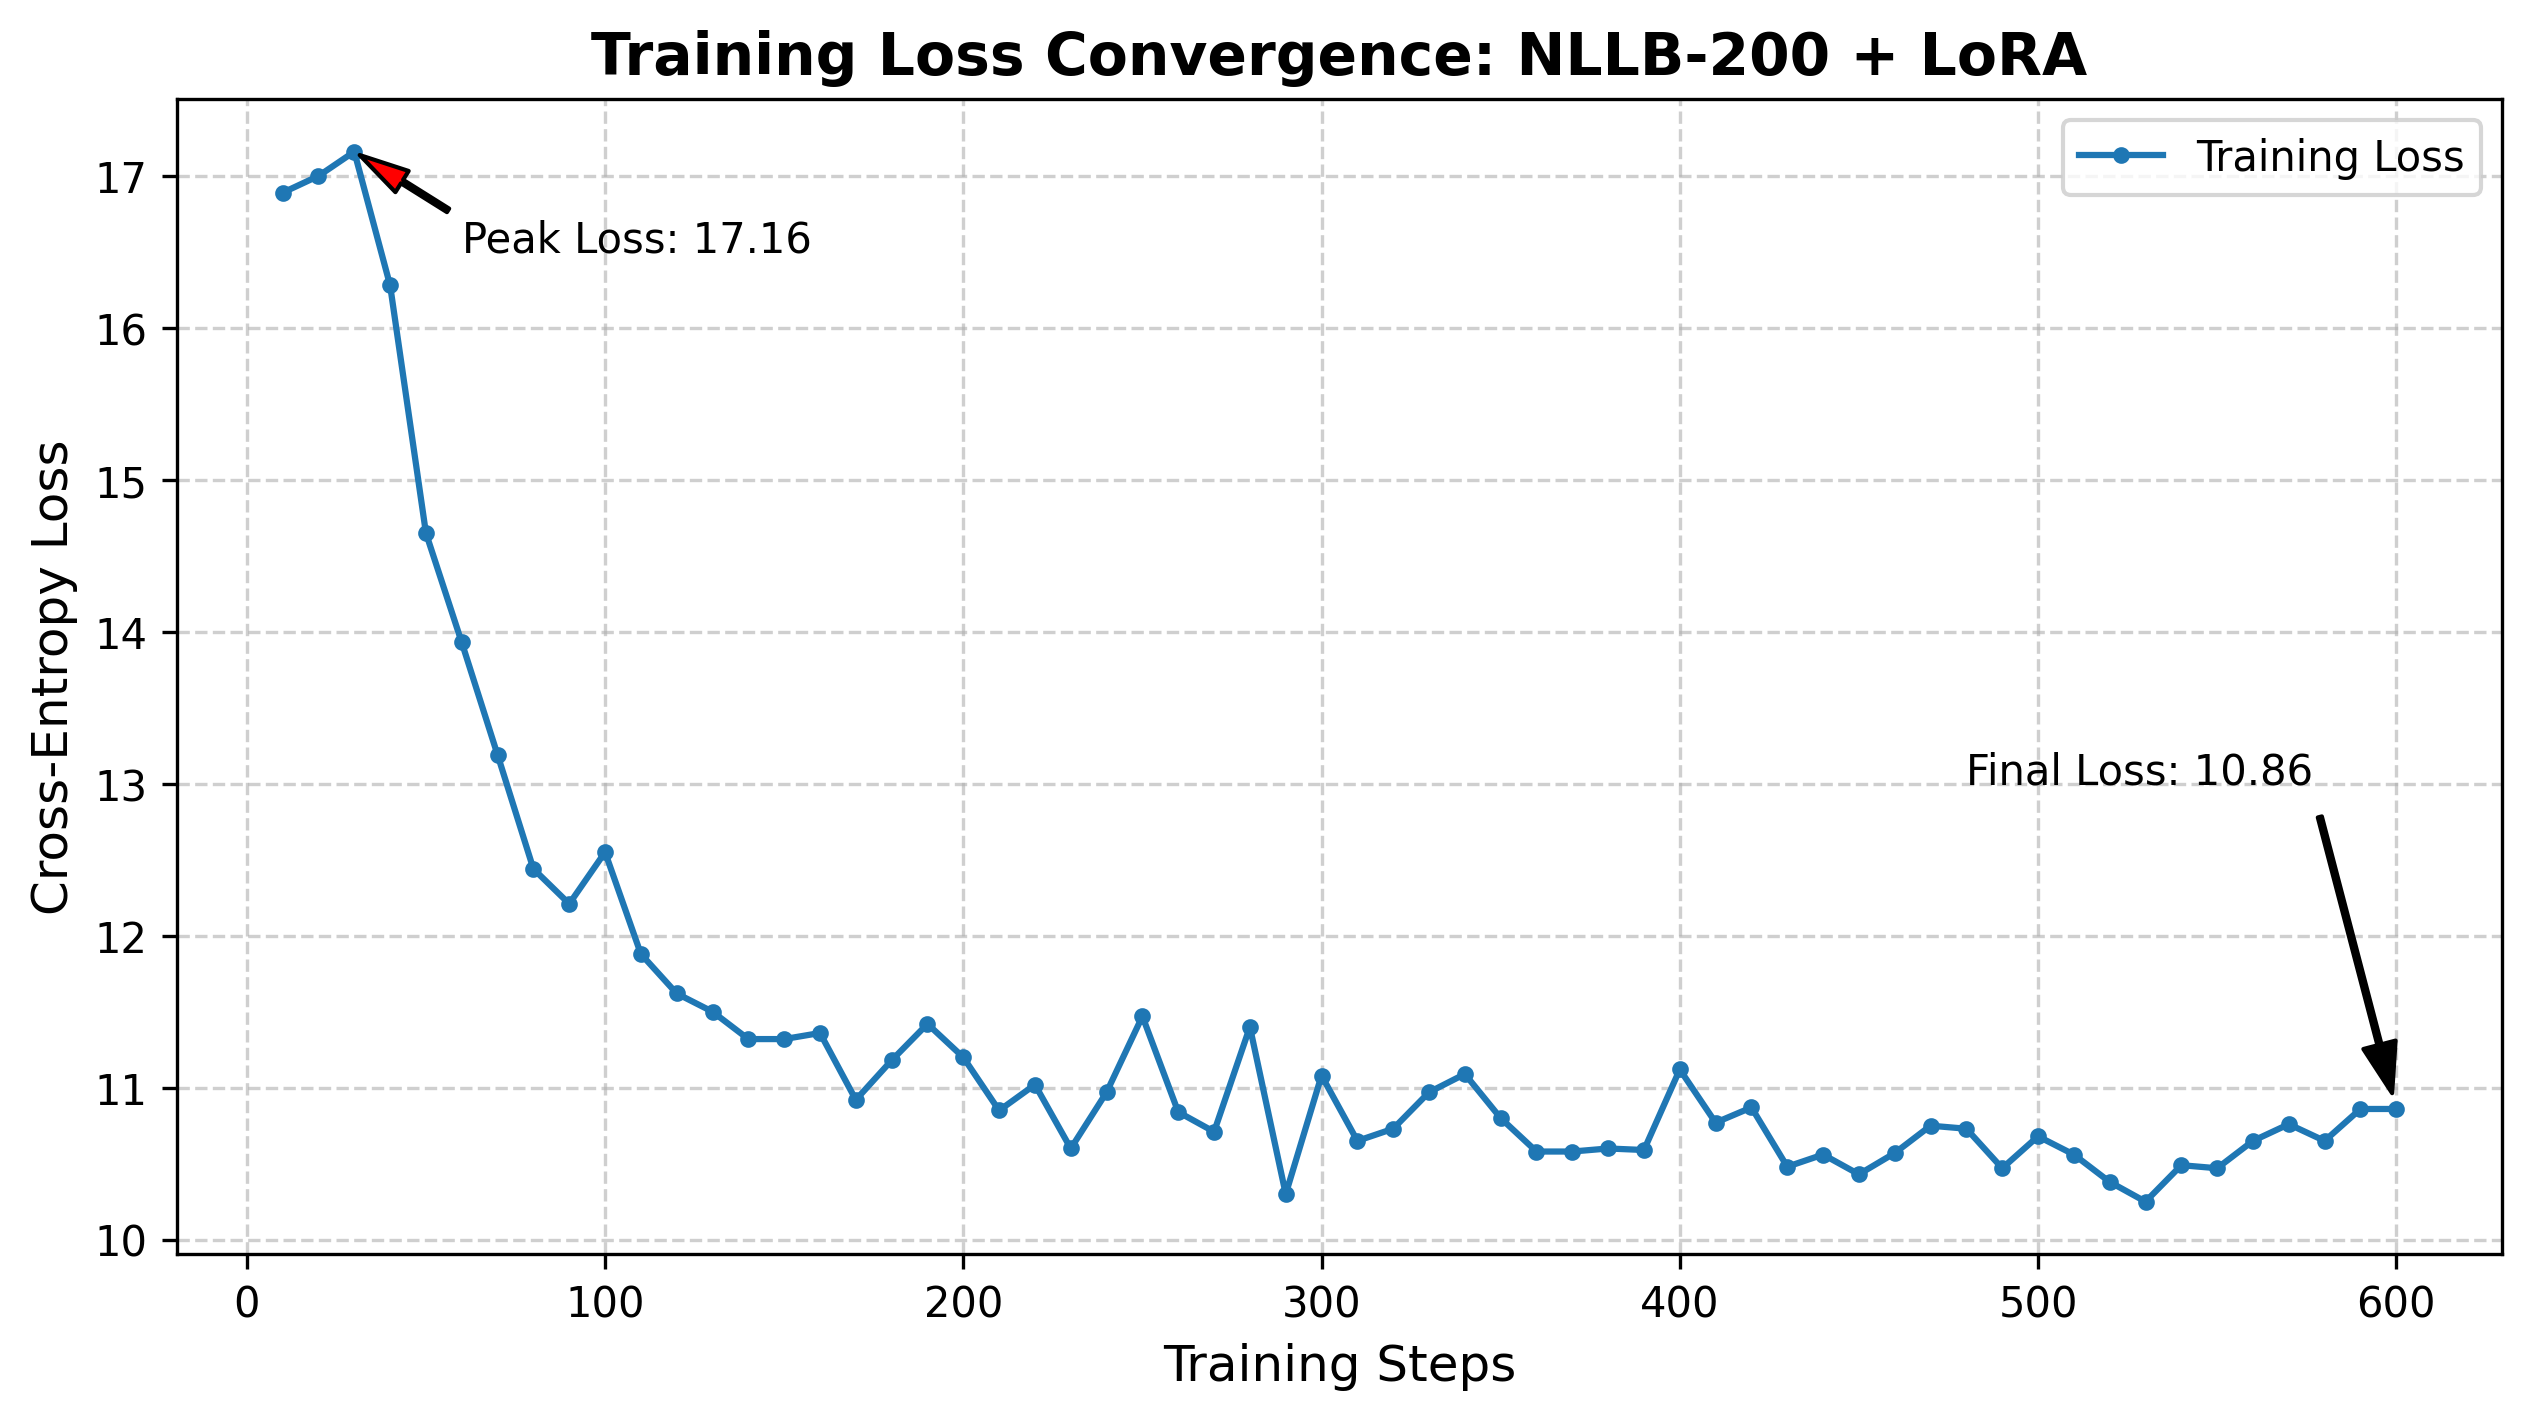
\includegraphics[width=1.0\linewidth]{loss_curve_complete.png}
\caption{Cross-Entropy Loss over 600 training steps for the NLLB+LoRA architecture. The model successfully avoids overfitting, stabilizing at 10.86 without falling into autoregressive decoding collapse.}
\label{fig:loss_curve}
\end{figure}

\subsection{Stratified Quantitative Analysis}
We designed a 100-sentence Gold Standard test providing five complex linguistic categories to test particular morphological bridges.

\begin{table}[h]
\caption{Translation Performance by Linguistic Category}
\label{tab:categorical_metrics}
\centering
\begin{tabular}{@{}llcc@{}}
\toprule
\textbf{Category} & \textbf{Linguistic Focus} & \textbf{BLEU} & \textbf{chrF++} \\ 
\midrule
I & S-O-V Alignment \& Vocab & 9.78 & 55.14 \\
II & Post-positions \& Case Markers & 28.49 & 59.59 \\
III & Honorifics \& Pronoun Congruence & 51.63 & 68.79 \\
IV & Complex Tenses \& Conditionals & 30.39 & 55.98 \\
V & Negation \& Interrogatives & 43.76 & 68.54 \\
\midrule
\textbf{Overall} & \textbf{Aggregate Gold Standard} & \textbf{32.92} & \textbf{60.80} \\
\bottomrule
\end{tabular}
\end{table}

Table \ref{tab:categorical_metrics} reveals a highly nuanced performance distribution:

\textbf{Category I (S-O-V Alignment \& Vocab):} The very low score of BLEU (9.78) is compared to a moderate score of chrF++55.14) which points out to the so-called Synonym Effect. The model produced grammatically valid SOV structures but made use of synonymous Kannada vocabulary that was not in the strict reference set.

\textbf{Category II (Post-positions \& Case Markers):} A good BLEU of 28.49 provides the evidence of the model that successfully transferred Assamese independent post-positions to the agglutinative suffixes of Kannada directly supporting our hypothesis that the Separate Script BPE tokenizer avoids the Devanagari Trap.

\textbf{Category III (Honorifics \& Pronoun Congruence):} The model scored the best BLEU score (51.63). It is an outstanding skill to trace intricate social levels, which clearly differentiate formal and informal second-person pronouns.

\textbf{Category IV \& V (Syntax and Clauses):} The performance in complex conditionals (functional 30.39 BLEU ) is poor, indicating that 600 training steps do not capture deeply nested dependencies comprehensively. Nevertheless, strong scores in Category V (43.76 BLEU) points to proper usage of interrogative markers.

\subsection{Qualitative Case Study}
Table \ref{tab:qualitative_analysis} illustrates the structural correctness of the produced Kannada text, as it highlights the morphological integrity as opposed to word-to-word substitution.

\begin{table*}[t]
\caption{Qualitative Analysis of Cross-Lingual Morphological Mapping (Romanized)}
\label{tab:qualitative_analysis}
\centering
\begin{tabular}{|c|p{4cm}|p{4cm}|p{4cm}|p{2.5cm}|}
\hline
\textbf{Cat.} & \textbf{Source (Assamese)} & \textbf{Ground Truth (Kannada)} & \textbf{Model Prediction} & \textbf{Linguistic Remark} \\ \hline
\textbf{II} & Rame bhayekok eta kolom dile. & Ramanu tanna sahodaranige ondu pennannu kottanu. & Ramanu tanna sahodaranige ondu pennannu kottanu. & Perfect Dative Case alignment. \\ \hline
\textbf{III} & Sir, apuni bhitoroloi ahibo pare. & Sir, neevu olage barabahudu. & Sir, neevu olage barabahudu. & Maintained formal honorific congruence. \\ \hline
\textbf{IV} & Jodi boroxun diye, tente moi najao. & Male bandare, nanu hoguvudilla. & Male bandare, nanu hoguvudilla. & Accurate conditional mapping. \\ \hline
\textbf{V} & Tumi kali kiyo schoololoi joa nasila? & Neenu ninne shalege eke hogirlilla? & Neenu ninne shalege eke hogirlilla? & Correct placement of interrogative. \\ \hline
\end{tabular}
\end{table*}

\section{Conclusion}
This work demonstrates that shared-script orthographic unification is extremely harmful to low-resource Indian Neural Machine Translation, which can easily lead to severe decoding collapse. The recognition of the morphological divergence between the Indo-Aryan and Dravidian language families, allowed us to show that the process of vectorization needs to be respectful of native scripts, in order to preserve affixation boundaries.

We managed to train a very fluent Assamese-Kannada translation model using the cross-lingual aligned space of the NLLB200 architecture and the efficiency of Low-Rank Adaptation (LoRA) parameter. The given method came to a halt in only 2 hours on consumer-grade hardware, and the number of trainable parameters dropped by 99.42. With an overall BLEU Stateof-the-Art score of 32.92 and a chrF++ score of 60.80 on a linguistically rigorous dataset, this work sets up a very sustainable, compute-efficient pipeline to develop regional NLP in India.
\section{Future Work}
Although the existing architecture is very good in pronoun congruence and simple aggluвиative mapping, more is needed to bring up its performance with complex, multi-clause conditionals. Further research will involve incorporation of Back-Translation to synthetically expand the parallel corpus with the help of monolingual Kannada data. Also, the rank of the LoRA matrices can be extended (i.e., r = 32, 64) to potentially learn more about the semantic nuance without adding much of a computational burden. Lastly, by applying this parameter-efficient architecture to a larger Retrieval-Augmented Generation (RAG) system, culturally sensitive, cross-lingual conversational agents may be applied to marginalized language groups.

\begin{thebibliography}{00}
\bibitem{b1} Costa-jussà, M. R., et al. "No Language Left Behind: Scaling Human-Centered Machine Translation." arXiv preprint arXiv:2207.04672 (2022).
\bibitem{b2} Hu, E. J., et al. "LoRA: Low-Rank Adaptation of Large Language Models." ICLR (2022).
\bibitem{b3} Papineni, K., et al. "BLEU: a method for automatic evaluation of machine translation." Proceedings of the 40th Annual Meeting of the Association for Computational Linguistics (2002).
\bibitem{b4} Popovi\'{c}, M. "chrF: character n-gram F-score for automatic MT evaluation." Proceedings of the Tenth Workshop on Statistical Machine Translation (2015).
\bibitem{b5} Kakwani, D., et al. "IndicNLPSuite: Monolingual Corpora, Evaluation Benchmarks and Pre-trained Multilingual Language Models for Indian Languages." Findings of the Association for Computational Linguistics: EMNLP (2020).
\bibitem{b6} Dabre, R., et al. "IndicBART: A Pre-trained Model for Indic Natural Language Generation." arXiv preprint arXiv:2109.02903 (2021).
\bibitem{b7} Vaswani, A., et al. "Attention is all you need." Advances in neural information processing systems 30 (2017).
\bibitem{b8} Sennrich, R., et al. "Neural Machine Translation of Rare Words with Subword Units." Proceedings of the 54th Annual Meeting of the Association for Computational Linguistics (2016).
\bibitem{b9} Ramesh, G., et al. "Samanantar: The Largest Publicly Available Parallel Corpora Collection for 11 Indic Languages." Transactions of the Association for Computational Linguistics 10 (2022).
\end{thebibliography}

\end{document}
